\documentclass{scrartcl}

\usepackage{
  cooltooltips,
  dtklogos,
  filecontents,
  geometry,
  graphicx,
  hyperref,
  lmodern,
  natbib,
  tikz
}

\geometry{
%  landscape,
  margin=1cm
}
\hypersetup{
  colorlinks=true,
  linkcolor=blue,
  urlcolor=blue,
  pdfborder=0 0 0
}

\def\XeT{XET}
\def\Aleph{Aleph}
\def\XeLaTeX{Xe\LaTeX}
\def\ConTeXt{Con\TeX{}t}
%\setmainfont{Linux Libertine}

\def\mynode#1#2#3#4{
  \node (#1) at (#2) {
    \cooltooltip{#1}{#3}{#3}{}{#4\strut}
  };
}
\newcounter{layer}\setcounter{layer}{0}
\def\setlayer#1{\setcounter{layer}{#1}}
\newcommand\steplayer[1][-1]{\addtocounter{layer}{#1}}
\pagestyle{empty}

\title{A short overview of \TeX\ and its children \dots}
\author{Arno Trautmann\thanks{arno.trautmann@gmx.de -- Please feel free to mail me any suggestions and comments!}}
\date{}

\begin{document}
\maketitle

\begin{abstract}
This paper tries to give a short overview of the development of \TeX. So far, most of the information is taken from the article \textsf{A brief history of \TeX, volume II} by Arthur Reutenauer in the proceedings of \textsf{EuroBacho\TeX 2007}. Additional information is taken from documentations (see references on page \pageref{sec:refs}). All information is up to the date of the generated pdf. Everything here is without guarantee -- this is just to get an overview. Consult the references for further (and/or correct) information!
\end{abstract}

\tableofcontents

\newpage
\section{\TeX\ -- the program, and extensions/derivatives}
\Large
\centering
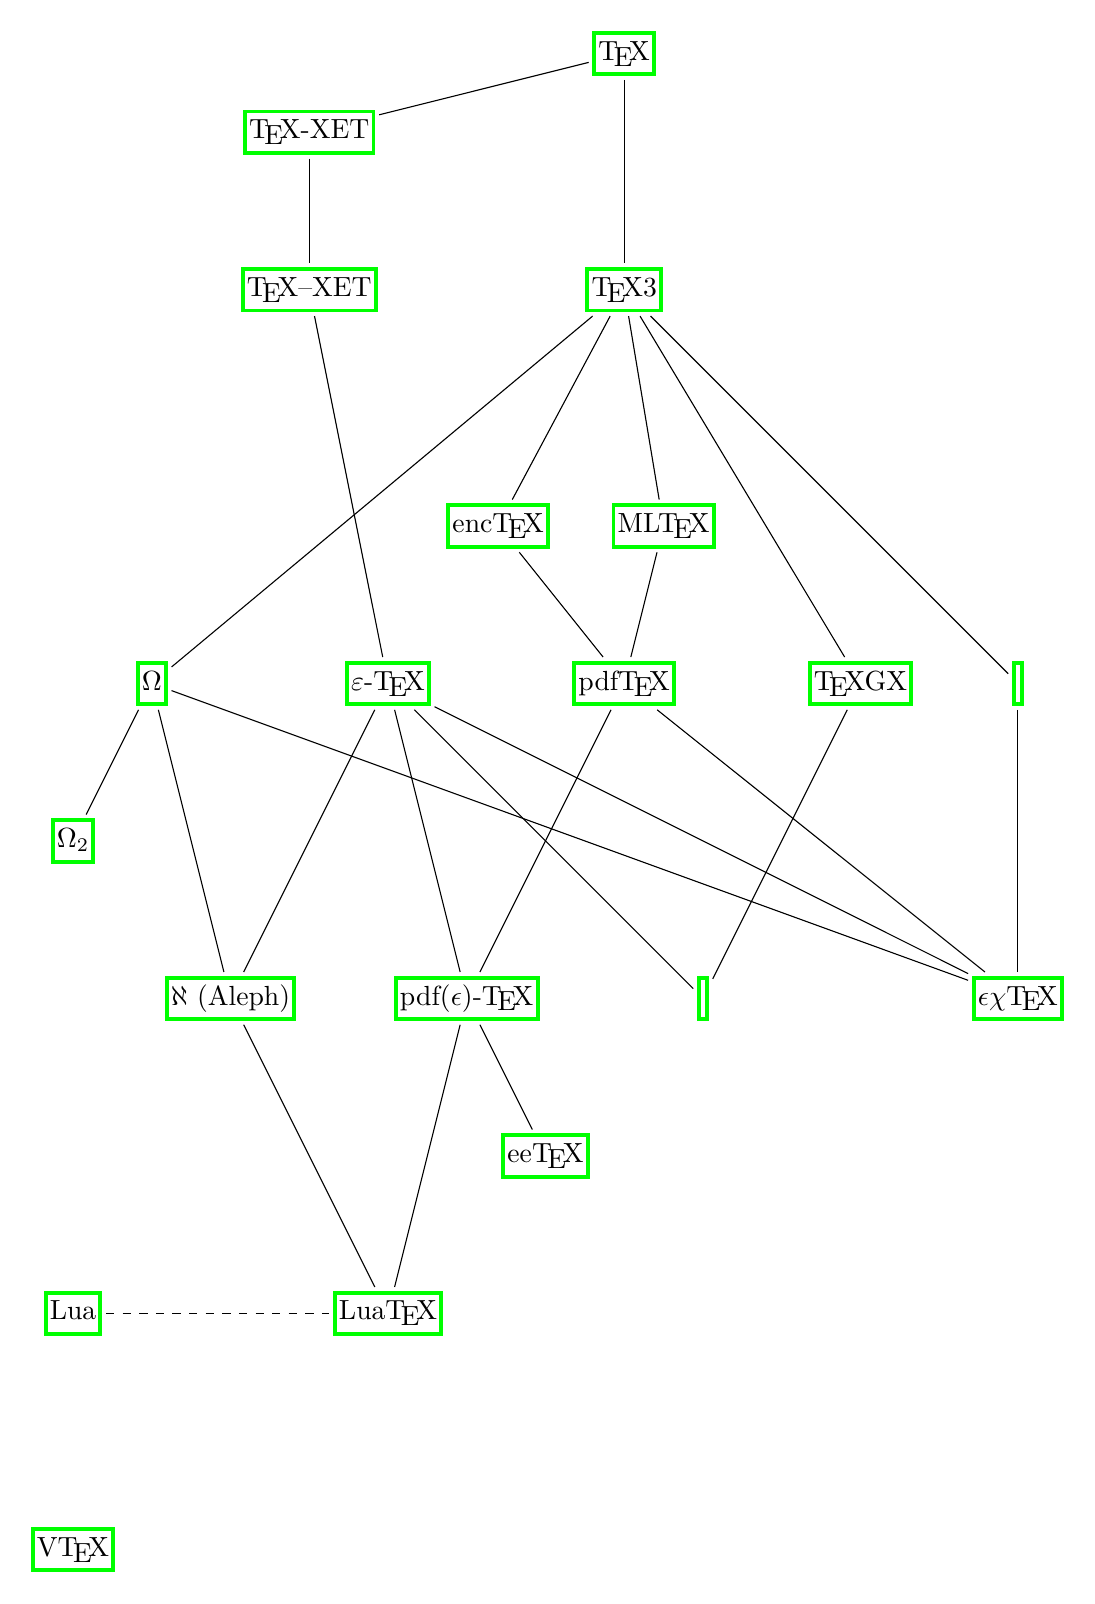
\begin{tikzpicture}
\setlayer2
\mynode{tex}{7,\thelayer}{born in 1978}{\TeX}

\steplayer
\mynode{xet-tex}{3,\thelayer}{The first extension to TeX, 1987. It was able to typeset in two directions, but only with a mark in the dvi to change the direction.}{\TeX-\XeT}
\draw (tex) to (xet-tex);

\steplayer[-2]
\mynode{xet--tex}{3,\thelayer}{TeX--XeT was able to really put the glyphs on the right place in the dvi.}{\TeX-{}-\XeT}
\draw (xet-tex) to (xet--tex);

\mynode{tex3}{7,\thelayer}{Ability to handle 8-bit input. 1989. TeX development was frozen in 1991.}{\TeX3};
\draw (tex) to (tex3);

\steplayer[-3]
\mynode{enctex}{5.4,\thelayer}{A small extension to TeX, started 1997. Adds 10 new primitives relating input re-encoding}{enc\TeX};
\draw (tex3) to (enctex);

\mynode{mltex}{7.5,\thelayer}{Extension (started 1990) to TeX that allows hyphenation of words with accented letters. Distributed as a change file to the original WEB sources of TeX.}{ML\TeX};
\draw (tex3) to (mltex);

\steplayer[-2]
\mynode{omega}{1,\thelayer}{Support for unicode-input. Still constrained on the output}{$\Omega$};
\draw (tex3) to (omega);

\mynode{etex}{4,\thelayer}{*the* extension to TeX.}{$\varepsilon$-\TeX};
\draw (xet--tex) to (etex);

\mynode{pdftex}{7,\thelayer}{A new engine to directly produce pdf-files from TeX, without the need of dvi-ps-pdf. This allows to use microtypographic extensions and many other features of the pdf format.}{pdf\TeX};
\draw (enctex) to (pdftex);
\draw (mltex) to (pdftex);

\mynode{texgx}{10,\thelayer}{?}{\TeX{}GX};
\draw (tex3) to (texgx);

\mynode{nts}{12,\thelayer}{A project to completely reimplement TeX in Java. Now NTS is officially declared dead.}{\NTS};
\draw (tex3) to (nts);

\steplayer[-2]
\mynode{omega2}{0,\thelayer}{A short-time try to pick up the development of Omega again in 2006. Seemed more like a good plan and is now regarded as obsolete. LuaTeX is kind of a successor.}{$\Omega_2$};
\draw (omega) to (omega2);

\steplayer[-2]
\mynode{aleph}{2,\thelayer}{originally named epsilon-Omega, an attempt to stabilize Omega while merging epsilon extensions.}{$\aleph$ (\Aleph)};
\draw (omega) to (aleph);
\draw (etex) to (aleph);

\mynode{xetex}{8,\thelayer}{This extension enables full multilingual support for left-to-right typesetting, right-to-left and almost any other possible direction. XeTeX also features support for OpenType and AAT-fonts.}{\XeTeX};
\draw (texgx) to (xetex);
\draw (etex) to (xetex);

\mynode{extex}{12,\thelayer}{Planned implementation of a high-quality typesetting system, written in Java. Based on experiences in NTS, eTeX, pdfTeX and Omega. Started in 2003, current version in repository is 0.0. (i. e. not very far ...)}{$\epsilon\chi$\TeX};
\draw (nts) to (extex);
\draw (omega) to (extex);
\draw (etex) to (extex);
\draw (pdftex) to (extex);

\mynode{pdfetex}{5,\thelayer}{Merging the pdfTeX engine with the eTeX-extensions. This engine can produce dvi (with or without the eTeX-extensions) as well as pdf (again, with or without extensions).}{pdf($\epsilon$)-\TeX};
\draw (etex) to (pdfetex);
\draw (pdftex) to (pdfetex);

\steplayer[-2]
\mynode{eetex}{6,\thelayer}{Experimental extension to pdfeTeX by Taco Hoekwater, created 2000. Distributed as change file.}{ee\TeX};
\draw (pdfetex) to (eetex);

\steplayer[-2]
\mynode{lua}{0,\thelayer}{Script language; has nothing to do with TeX!}{Lua};

\mynode{luatex}{4,\thelayer}{Still in heavy active development, LuaTeX will support unicode, OpenType and totally everything. It features an embedded scripting language, lua, making it easy to extend.}{Lua\TeX};
\draw (aleph) to (luatex);
\draw (pdfetex) to (luatex);
\draw[dashed] (lua) to (luatex);

\steplayer[-3]
\mynode{vtex}{0,\thelayer}{Please insert information here ...}{V\TeX};

\end{tikzpicture}



\newpage
\section{\LaTeX\ (Lamport's \TeX) -- a format and large macro package for \TeX}
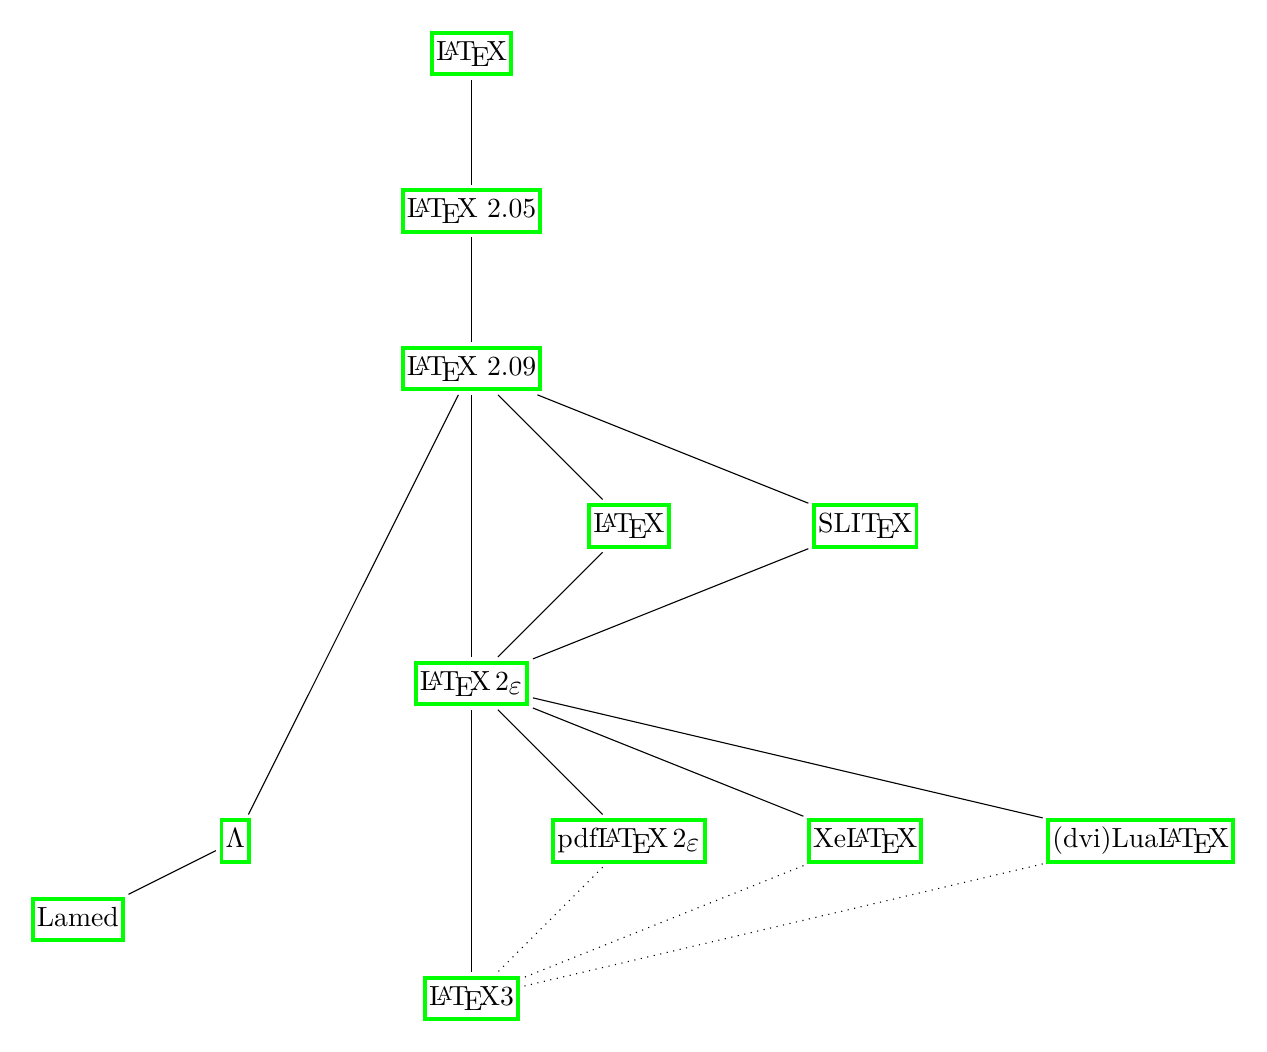
\begin{tikzpicture}
\mynode{latex}{0,2}{Inofficial versions? …}{\LaTeX};

\mynode{latex205}{0,0}{? …}{\LaTeX\ 2.05};
\draw (latex) to (latex205);

\mynode{latex209}{0,-2}{The first official version by Leslie Lamport, 1985.}{\LaTeX\ 2.09};
\draw (latex205) to (latex209);

\mynode{amslatex}{2,-4}{A variation of LaTeX2.09 aiming for high quality math typesetting.}{\AMS\LaTeX};
\draw (latex209) to (amslatex);

\mynode{slitex}{5,-4}{A variation of LaTeX2.09 to provide an easy way for producing presentations.}{SLI\TeX};
\draw (latex209) to (slitex);

\mynode{latex2ε}{0,-6}{New release of LaTeX to avoid incompatible dialects of LaTeX 2.09.}{\LaTeXe};
\draw (latex209) to (latex2ε);
\draw (amslatex) to (latex2ε);
\draw (slitex) to (latex2ε);

\mynode{pdflatex}{2,-8}{The standard LaTeX. If anyone talks about "LaTeX" it is nearly shure to be this package. pdfLaTeX2e produces pdf or dvi output.}{pdf\LaTeXe};
\draw (latex2ε) to (pdflatex);

\mynode{xelatex}{5,-8}{Using the XeTeX engine. There are some special packages that provide easy access to the modern features of XeTeX.}{\XeLaTeX};
\draw (latex2ε) to (xelatex);

\mynode{lualatex}{8.5,-8}{LaTeX based on LuaTeX with pdf (standard) or dvi (dviLuaLaTeX) output.}{(dvi)Lua\LaTeX};
\draw (latex2ε) to (lualatex);

\mynode{lambda}{-3,-8}{A LaTeX-package for the omega-engine.}{$\Lambda$}
\draw (latex209) to (lambda);

\mynode{lamed}{-5,-9}{A LaTeX-package for the aleph-engine.}{Lamed}
\draw (lambda) to (lamed);

\mynode{latex3}{0,-10}{The planned successor of LaTeX2e. It is planned to implement a very elaborate low-level programming language. The expl3-package provides a test-implemantation that can be used in LaTeX2e.}{\LaTeX{}3};
\draw (latex2ε) to (latex3);
\draw[dotted] (xelatex) to (latex3);
\draw[dotted] (pdflatex) to (latex3);
\draw[dotted] (lualatex) to (latex3);
\end{tikzpicture}


\newpage
\section{\ConTeXt\ -- the other major format and \TeX\ macro package}
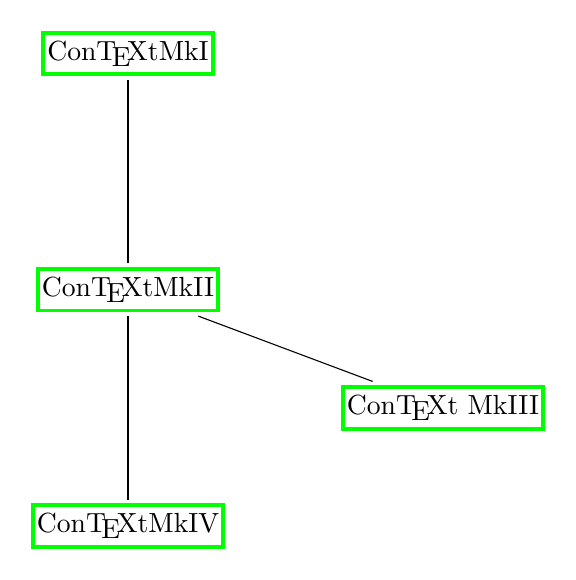
\begin{tikzpicture}
\mynode{mki}{0,0}{Original ConTeXt with Dutch low level interface.}{\ConTeXt MkI};
\mynode{mkii}{0,-3}{ConTeXt with English low level interface. Works with any TeX-engine, like LaTeX: TeX, e-TeX, pdfTeX, Aleph, XeTeX, ...}{\ConTeXt MkII};
\draw (mki) to (mkii);

\mynode{mkiii}{4,-4.5}{Reserved for future use for files supporting XeTeX. Has not been used yet.}{\ConTeXt\ MkIII};
\draw (mkii) to (mkiii);

\mynode{mkiv}{0,-6}{Specially designed for LuaTeX.}{\ConTeXt MkIV};
\draw (mkii) to (mkiv);
\end{tikzpicture}

\newpage
\section{\TeX's "little" helpers}
\parbox{\textwidth}{This is a small section to mention programs that are very helpful and specially designed to support the work with \TeX.}\vspace{3ex}


\begin{tikzpicture}
\mynode{mki}{0,0}{Very helpful and important tool for creating bibliographies.}{\BibTeX};
\end{tikzpicture}
%%
%% I've chosen to typeset the bibliography "by hand" as to avoid problems regarding formatting. And this way I only need one file.
%%
\newpage
\normalsize
\begin{thebibliography}{10}
\refstepcounter{section}
\label{sec:refs}
\bibitem[{Annotations}()]{}{\quad The references are in order of occurance in the above document. I.\,e. if you want information about Lua\TeX, it will be below e.\,g. $\epsilon$\TeX.}

\bibitem[{Books}()]{}{\large\textbf{\textsf{Books}}}

\bibitem[Knuth et~al.(1986)Knuth, Bibby, and Makai]{knuth1986texbook}
D.E. Knuth, D.~Bibby, and I.~Makai.
\newblock \emph{{The \TeX book}}.
\newblock Addison-Wesley Reading, MA, 1986.

\bibitem[Mittelbach et~al.(2004)Mittelbach, Goossens, Braams, Carlisle, Rowley,
  Detig, and Schrod]{mittelbach2004latex}
F.~Mittelbach, M.~Goossens, J.~Braams, D.~Carlisle, C.~Rowley, C.~Detig, and
  J.~Schrod.
\newblock \emph{{The \LaTeX\ companion}}.
\newblock Addison-Wesley, 2004.

\bibitem[{WebEngines}()]{}{\large\textbf{\textsf{Web Sources (Engines)}}}

\bibitem[{ML\TeX\ source}()]{mltex}{ML\TeX\ source (CH file)}
\newblock \url{http://www.tex.ac.uk/tex-archive/systems/generic/mltex/mltex.ch}

\bibitem[{enc\TeX\ page}()]{enctex}
{enc\TeX\ page}
\newblock \url{http://www.olsak.net/enctex.html}

\bibitem[{\NTS\ project page}()]{nts}
{\NTS\ project page}
\newblock \url{http://nts.tug.org}

\bibitem[{$\epsilon\chi$\TeX\ project page}()]{extex}
{$\epsilon\chi$\TeX\ project page}
\newblock \url{http://www.extex.org}

\bibitem[{ee\TeX\ project page}()]{eetex}
{ee\TeX\ project page}
\newblock \url{http://tex.aanhet.net/eetex}

\bibitem[{omega and aleph}()]{omegaleph}
{short article about omega and aleph}
\newblock \url{http://www.tex.ac.uk/cgi-bin/texfaq2html?label=omegaleph}

\bibitem[{Lua\TeX\ project page}()]{luatex}
{Lua\TeX\ project page}
\newblock \url{http://www.luatex.org}



\bibitem[{WebMakro}()]{}{\large\textbf{\textsf{Web Sources (Makro Packages/Formats)}}}
\bibitem[wiki()]{contextgarden}
\ConTeXt\ wiki
\newblock \url{http://wiki.contextgarden.net}

\bibitem[{\LaTeX\ project page}()]{latexproject}
{\LaTeX\ project page}
\newblock \url{http://www.latex-project.org}

\bibitem[{\LaTeX3 project}()]{latexprojectiii}
{\LaTeX3 project}
\newblock \url{http://www.latex-project.org/latex3.html}

\end{thebibliography}


\end{document}